\documentclass[12pt]{article}
\usepackage{soul}
\usepackage{graphicx}
\usepackage{url}

\title{Design Document for a Microgrid Simulation}
\author{Dan Gordon}
\date{\today}
\begin{document}
\maketitle

%\begin{abstract}
%\end{abstract}

\section{High-level brief} Implement a detailed level simulation of microgrids, or elements of microgrids, that will be suitable for research into optimisation.

\section{Types of users}

\begin{description}
\item[Researcher non-programmer] A typical ``user'' who just wishes to use a product without being involved too heavily in the nuts and bolts. 
\item[Researcher programmer] Doing research primarily into optimization strategies for the microgrid or smart grids. Is comfortable with writing code e.g. that makes use of an API, implements program hooks etc. 
\item[Support programmer] Someone who has a high degree of ownership over the code, and who may be asked at any time to implement new features, e.g. writing a new controller or appliance, for use by other users.
\end{description}

\section{Process use cases}
Detailed use cases for the simulator will depend on what the user wishes to achieve (e.g. what is the optimisation or testing process) as well as on the model that is being explored by the user. When considering how the simulation will be used, it is helpful to separate these two aspects of the simulation. Below, we consider the process without specifying the model.

\begin{description} 

\item[Simple Simulation] Researcher wants to evaluate the effectiveness of one or more MG models, using standard components and controllers. Sets up model using a standard interface, and runs simulation.

\item[Parametrically Customizable Controllers] Researcher explores parameter space for controllers, using already existing smart controllers, where decision variables are controller parameters.

\item[Custom Controllers] Researcher wants to evaluate the effectiveness of custom algorithms for controlling the components of a MG. Writes custom code for controllers that can be linked to the main simulator. Sets up simulation and runs.

\item[Simulation in Optimization] Researcher wants to employ machine learning techniques to train microgrid controllers. Writes controllers that interface with the simulation. Writes ML code that calls the simulation. Runs ML code.

\end{description}

\section{Elements of the problem domain}
We will now move on to consider the different kinds of models that might be employed within the simulator. We start by listing the important elements of these models.

\begin{description}

\item[Grid objects] Lines, transformers, etc.

\item[House objects] Thermal properties of houses, data about occupants, etc.

\item[Appliances] HVAC, electric HW, lights, other appliances.

\item[DER generators] PV generation, wind generation, fuel cells, diesel generators, etc. 

\item[DER storage] Batteries, thermal storage, other? 

\item[Smart meter in house] Receive directive from microgrid or utility e.g. price per kW/h or information related to fault. [Directives could be economic/suggestions/mandatory instructions].

\item[Smart appliance controllers]
Receive directive from smart meter. Schedule appliance.

\item[Smart controllers for microgrid sources and storage] Receive (general) directives from overall MG controller. Sense network voltage etc. Control device to which they are attached.

\item[Smart controllers for microgrid] Receive information (e.g. price per kW/h, faults) from utility. Sense local electricity supply e.g. voltage fluctuations. Decide when to island. Dispatch directives to plug-and-play microgrid components. Exercise control over individual radial feeders in MG.

\item[Climate and weather] This is crucial for realistic modeling of house performance.

\item[Market] Model or data for electricity demand and price.

\end{description}

\section{Models for use cases}
Having specified the elements, we now describe some typical classes of models that could be employed.

\begin{description}

\item[Smart house with DR] House, including panel for connection to grid using single phase 240 V power.  Contains circuits with appliances. There is a smart meter to the house that is able to provide simple directives from the utility: at first instance, just current cost per kW/h. The smart meter will also have access to information about averaged cost schedules\footnote{A schedule specifies an object that varies periodically as a function of time. A typical example might be cost of power, as a function of the weekday and time of day.}, so that it might predict future demand. Appliances may be connected to private or shared controllers (customizable by the user) that is also connected to the smart meter. Controllers could either directly tell applicances when to switch on or off, or instead they could have access to the set points of the appliance.

\item[Smart house with generation and/or storage?]

\item[Grid-connected typical small microgrid with DR at microgrid level] Use model from Chowdhury, Chowdhury and Crossley, \ul{Microgrids and Active Distribution Networks}. Loads could be treated in a simplified manner e.g. using a typical voltage and power profile / ZIP loads. The microgrid is connected to the grid which is represented as a slack bus i.e. constant voltage and phase. There is a microgrid controller that is able to receive information from the utility. Initially, this could be just a price per kW/h. Later, it might be possibly to also incorporate small fluctuations in voltage and reactive power that may be sensed at the point of connection to the microgrid, or stochastic fault modelling.  Each generater source also has an independent controller, which is able to sense local fluctuations in voltage [phase? reactive power?] as well as receive and/or send to the microgrid controller. There are limitations, however, on the nature of this communication because the microsources are designed to be plug-and-play.

\begin{figure}
\begin{center}
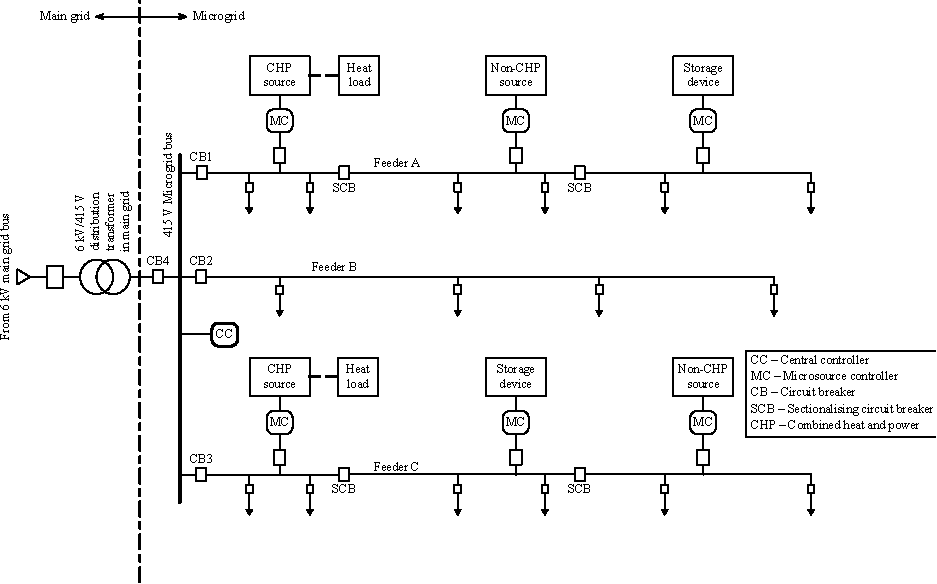
\includegraphics[width=11cm]{MGSchematic.pdf}
\caption{A typical microgrid configuration. Figure taken from Chowdhury, Chowdhury and Crossley, \ul{Microgrids and Active Distribution Networks}.}
\end{center}
\end{figure}

\item[Islanded microgrid] Similar to above, but the microgrid is now no longer connected to the grid. We need to flesh out what needs to be optimized here. Clearly, we will aim to run for as long as possible, and there will be some kind of hierarchy of critical loads. Given the requirements decided on, we'll need to decide on how the architecture copes. Presumably this will happen at the level of the overall microgrid controller telling which sources to turn on and off? Also, we need to bear in mind that islanding a microgrid may play havoc with standard methods for solving powerflow equations. For example, how well will Gridlab-D cope with this situation (see below)?

\item[Microgrid with faults on utility side] Long term simulations of a microgrid, where faults can occur on the utility side. The focus of optimisation is on optimal charging and use of storage devices, and on optimal [firm up the ideas here] operation of the grid after a fault occurs. 

\item[Microgrid with faults on microgrid side]

\item[Microgrid with CHP] Concentrate on the microgrid architecure and/or control, to obtain most energy efficient heating of houses. For example, CHP can be driven by the need for electricity generation (in which case, too much or too little heat may be generated), or by the need for heat generation (in which case, too much or too little electricity may be generated.

\item[Aggregate model] Aggregate items above - e.g. microgrid with smart houses in grid-connected mode. Model could get as complex as desired.

\end{description}

\section{Development Options}

Here, we begin to consider some of the high level decisions that will need to be made before starting the real development process. A major roadblock to developing the simulation is the complexity of the components required to do detailed modelling, and the limited developer resources available. I suggest that there are two questions that should be considered at a very early stage
\begin{enumerate}
\item What level, or granularity, of modelling will be sufficient for our needs? What are the implications of using simplified models? Can we live with that?
\item Should we leverage pre-existing open source software? If so, which software and how? What will be the advantages and disadvantages for our simulation? 
\end{enumerate}
These two questions are related, because choosing to use pre-existing software will give us access to models that have already been developed, and the choice of software will naturally depend on whether it is capable of modelling at our chosen granularity. The first question can be broken down into specific questions
\begin{enumerate}
\item What is the maximum level of detail at which we would like to model a house? A full thermal model, incorporating the weather, mass effects of the house etc.? Or a simple aggregated load schedule that just draws on typical usage profiles? The former would allow a detailed model of smart appliances, while the latter might be sufficient for modelling certain aspects of the overall operation of the microgrid.
\item What level of detail should the powerflow be modelled at, within the microgrid? At the highest level of detail, all transformers, lines etc. would be modelled, and at the lowest level, only the real power would be considered and the network topology might not even come into play. The detailed model would allow things like voltage stability, reactive power, overvoltages and overcurrents to be considered, while the simplified model would concentrate on the use of resources e.g. battery charging, switching on and off of generator sources etc.  \item Finally, what time/frequency granularity is needed? Specifically, do we need to be able to consider transients and harmonics? Slower frequency drift? Or can we assume that only slow changes in the voltage and phase angle need be considered, with frequency being essentially considered a constant?
\end{enumerate}

Given these two questions, the following courses of action might be taken:

\begin{enumerate}

\item Write the simulation from scratch, at a detailed level of modelling. Realistic models need to be implemented for buildings, appliances, DER devices and the grid itself. Each model will need a large investment of developer time.  Therefore, within a year and using one programmer, we might hope to implement a limited subset of all the tasks. This could be prioritised, e.g. concentrate on just an grid-connected microgrid with one or two forms of generation and storage. This would still be quite challenging.  
\item Write the simulation from scratch, but abandon the requirement to detailed level modelling. Instead, implement some kind of simplified model that concentrates on the omtimisation aspect while using a more approximate model of the power and heat flow.  
\item Borrow freely from open source software to create components, while still writing the overall architecture of the program from scratch. This has the advantage of providing excellent flexibility. The pitfall is the extra work needed.  There will also be a fairly large investment in converting the borrowed components to the architecure of the simulation.  Nonetheless, this would still be much more efficient than implementing all the models from scratch.
\item Modify an open source software package to suit our needs. For example, custom controllers could be implemented in Gridlab-D, and/or the process for modifying or developing new controllers could be well documented and made available to researchers. Other modifications to the package (for example, implementing 1-phase 240 V household circuits in Gridlab-D, which is currently designed around the US-style split phase 120/240 V circuits) will probably also need to be carried out.  
\item More or less, just use a piece of open source software and see how far we get with it.  
\end{enumerate}

\section{Gridlab-D} At present, I would suggest that the standout open-source software package that might suit our purposes is Gridlab-D. A few other options are available, such as OpenDSS or Matpower. I would tend to reject OpenDSS, because it is written in Delphi, is suitable only for Windows, and concentrates more on the traditional power flow problem and less on future smart grid technologies. Matpower is written in Matlab, which has various advantages and disadvantages. I believe it is also aimed more at the traditional power flow problem. I believe it has been ported to Python. It could perhaps be a candidate for further consideration.  Gridlab-D was designed with a similar aim to this project: simulation of the smart grid at a level that includes detailed modelling of enduses. However, it is only just at the cusp of gaining a full ability to model microgrid technologies. At present, many of the micro power sources have been implemented and are available, and the ability to model situations like an islanded microgrid is currently in development [TODO - a detailed list of what is and what isn't possible].  
\subsection{Code}
The Gridlab-D source code is written in a combination of C and C++. The core engine is C, while many of the modules are C++. While having the core implemented in C provides a high degree of flexibility (e.g. modules can be written in several different languages and easily linked with the core), it means that the syntax for handling generic variables in the simulation is somewhat long-winded and a bit harder to work with.

The code is open source, and is reasonably well documented. It compiles on several platforms e.g. Windows, MacOS, Linux. 

\subsection{Powerflow solvers and simulation architecture} 
Gridlab-D employs an agent-based approach to simulation.  Each simulation object can act as an independent agent in the simulation. Objects have (read only or read/write) access to a set of variables that are ``published'' by other objects \footnote{I think that these objects must be parent objects of the given object.  There is some kind of topological
constraints that govern the flow of information at each step, but I'm very hazy about how it all fits together at this stage. There seems to be various passes, based on the tree ordering of objects.  Each object has a rank, with the lowest ranked object being the trunk of the tree. I think there is a first topdown pass, a bottom up pass and a second topdown pass. Corresponding to these are presync, sync and postsync functions for each object. I think this is all a function of the forward-backward sweep solution method, so I don't know what happens when Newton-Raphson is used. See \url{http://www.gridlabd.org/documents/doxygen/1.1/group/powerflow.html}}

At each timestep, each object is asked to carry out a ``synchronize'' operation. The input to the synchronize function is the time $t_0$ of the previous synchronisation (i.e. the object's previous timestep, the time to which it is synchronised before the synchronize function has done any work) and the time $t_1$ which the object is being asked to update its state to (``now''). The output is the time at which the updated object is then expected to undergo its next state change, under the assumption that the states of all other related objects in the simulation remain fixed to their state at $t_0$. For example, if the object is a hot water heater, the time of the next state change might be the projected time at which the heating element turns off, as calculated by applying heat flow equations and taking into account the setpoints of the controller. The simulation then progresses to the time of the earliest projected state change for all the objects in the simulation. Synchronise is then called again, using the previous $t_1$ as the current $t_0$ and the time of the earliest state change as $t_1$. This loop then continues until the simulation ends. At a given synchronisation step, the current time $t_1$ might be returned by an object, signifying that its next state change will be immediate. In this case, the main simulation clock will not advance in the current iteration.  The objects in the simulation will update their states, and synchronize will be called again and again iteratively until either the simulation clock advances or a maximum number of iterations is reached. [In the latter case, the simulation ends with and error? It seems that there is the possibility of endless loops occurring here - perhaps this is why a parent child structure is imposed on the hierarchy of objects? More information needed.].

\subsection{Extesibility}

The architecture of Gridlab-D supports a degree of extensibility. For example, a device controller could be written that has access to the setpoints of a given device, and adjusts these over the course of a simulation \footnote{PLC controller prior to v. 3.0, PID controller as of v. 3.0}. This could be done without chaning the code in the device itself. Development versions of the program include hooks for incorporating external code within the simulation run loop, and for incorporating simulation runs within external code. The caveat is that these features are undergoing current development and change, so a stable way of using some of these features does not really currently exist. This is not to say that it can't be done, or that the ability to do so can't be easily added, only that in the near future the preferred way of doing so may change.

Here are some use cases for adding extensions to Gridlab-D, at the user level: \begin{enumerate}
\item A new appliance is required. The user, who is comfortable with programming in C++, writes a new appliance object class.  She starts with a similar existing appliance class, copies the source code, and changes the code where needed. The new class is separately compiled and linked into the Gridlab-D executable at runtime, using dynamically linked libraries [TODO - not sure about this].
\item A new appliance controller is required.\footnote{While this could be tackled by writing a new appliance, it is desirable to separate the implementation of the appliance from the controller. The appliance object responds to its settings e.g. heating and cooling setpoints, while the controller is responsible for tweaking these settings.} The user writes a controller object that refers to the published variables of both the appliance and other objects (e.g. - the setpoints of the HVAC, and the air temperature of the house). The new controller is linked at runtime to the simulation.
\item A new microsource controller is required. Flow proceeds similar to appliance controller above.
\item Ditto for a new microgrid controller.
\item An algorithm has been designed to train an optimisation algorithm or smart controller. Gridlab-D is to be used to generate data for the algorithm, with each run adding a data point. The algorithm is coded in C++. It uses links to Gridlab-D via an API. Gridlab-D simulations are therefore run from within the overarching structure of the training algorithm. [TODO - I have very little idea of what features of Gridlab-D would be leveraged to do this].
\item There are provisions in GLD for including C++ code in the configuration file, that is compiled dynamically at runtime. I need to find out more about this. I strongly suspect it will only work on Windows platforms.
\end{enumerate}

\subsection{Problems} 

One issue that exists for Gridlab-D is the ubiquitous use of US-style split-phase household circuits. The Gridlab-D house model includes a US-style ``panel'' object. This panel is currently only able to connect, on the distribution side, to a transformer that will not be appropriate to Australia or Europe. Appliances are either 120 V or 240 V, depending on whether they use a p-n or p-p circuit. Fortunately, the HVAC (and, I believe, the hot water heating) appliances are 240 V. The HVAC is the most complex appliance, because it directly interacts with the physics of the house. To run Gridlab-D with residential level modelling, something would need to be done about this situation. A user group discussion [TODO: reference?] implies that modifying the transformer would be the hardest part, because details of the transformer are used in the Newton-Raphson solver itself. It could be done, but would be far from trivial. In the same discussion, one or two possible workarounds are given, although these are not ideal. This discussion was initiated by one Jack Dangar from Ausgrid, who apparently developed his own house model. It would probably be worth getting in touch with him before tackling this issue.  Another issue is the question of islanding. [TODO I am not certain of this], but it is possible or even probably that the powerflow solvers will require a slack bus somewhere in the network. If this is the case, then the only way to model islanded microgrids in a reasonable manner would be to write a new powerflow solver.  
\section{Questions}
\begin{enumerate}
\item Which development course should we take?
\item At what level of complexity should the network and loads be modelled?
\item Do we want to consider transients? Power quality/harmonics?
\item Which of the process use cases will apply? Are there any others? Comments?
\item Which example models will apply? Are there others? Comments?
\item We should develop some detailed use cases for optimisation. This is best done with input from potential users of
the software.
\end{enumerate}

\section{Suggested course of action - to be discussed}
\begin{enumerate}
\item Develop a single detailed use case / scenario, and several less detailed ones.
\item Try to model the former in Gridlab-D.
\item Work out what needs to be added to make it work. Bear in mind the less detailed cases, to avoid developing a
solution that is too specific and will need to be abandoned.
\item Implement the solution. At this point, we will have a better idea of how Gridlab-D works and what will be needed
for developing the tool we want.
\item Write some tests
\item Flesh out the design for the tool
\item Implement aspects of the design iteratively, using the tests at each
stage. 
\end{enumerate}

\section{Appendix}
\subsection{Notes included as an aide-m\'emoire}
GLD - transactive controller object - simple way of doing DR for appliances.  Hooks up to an auction object etc. Has 5 properties from connected objects: set point, observation, power demand, load power, total power. Use this as a starting point when writing DR controllers. 

Schedule - create arbitrary load or other schedules. Can be used to customize devices etc.

Slack bus problem. Classic power flow problem specifies PQ for loads and PV for generators.

\end{document}
